\documentclass[11pt,a4paper]{article}

% ---------------------------------------------------------------- packages
\usepackage[utf8]{inputenc}
\usepackage[T1]{fontenc}
\usepackage{lmodern}
\usepackage{amsmath,amssymb}
% Small math symbols use the 8pt design so the report builds from a minimal font set.
\DeclareFontFamily{OMS}{lmsy}{\skewchar\font48 }
\DeclareFontShape{OMS}{lmsy}{m}{n}{<-8.5> lmsy8 <8.5-9.5> lmsy9 <9.5-> lmsy10}{}
\usepackage[top=2.3cm,bottom=2.3cm,left=2.5cm,right=2.3cm,headheight=14pt]{geometry}
\usepackage{graphicx}
\usepackage{xcolor}
\usepackage{booktabs,tabularx,array,float}
\newcolumntype{L}{>{\raggedright\arraybackslash}X}
\usepackage{enumitem}
\usepackage{fancyhdr}
\usepackage{titlesec}
\usepackage{caption}
\usepackage{placeins}
\usepackage{listings}
\usepackage{microtype}
\usepackage{tcolorbox}
\tcbuselibrary{skins,breakable}
\usepackage[linesnumbered,ruled,vlined]{algorithm2e}
\usepackage{tikz}
\usetikzlibrary{arrows.meta,positioning,calc,decorations.pathreplacing}
\usepackage[colorlinks=true,linkcolor=black,citecolor=black,urlcolor=black]{hyperref}
\hypersetup{pdftitle={Reaction-Diffusion Population Dispersal - Project Report},
  pdfauthor={Diya Patel, Abhiram Dodla, Aum Vijay Bawiskar, Divyanu Singh, Anshuman Singh, Druhin Sourya Datta Bommisetti, Akash Tejas Jog}}

% ---------------------------------------------------------------- layout
\setlength{\parindent}{0pt}
\setlength{\parskip}{5pt plus 1pt minus 1pt}
\renewcommand{\arraystretch}{1.25}
\setlist{nosep,leftmargin=*,topsep=3pt,itemsep=2pt}
\setcounter{tocdepth}{2}
\captionsetup{font=small,labelfont=bf,labelsep=period,skip=6pt}
\raggedbottom
\setlength{\emergencystretch}{3em}

\pagestyle{fancy}
\fancyhf{}
\fancyhead[L]{\small\itshape Reaction-Diffusion Population Dispersal --- Project Report}
\fancyhead[R]{\small Group Project}
\fancyfoot[C]{\small\thepage}
\renewcommand{\headrulewidth}{0.4pt}
\fancypagestyle{plain}{\fancyhf{}\fancyfoot[C]{\small\thepage}\renewcommand{\headrulewidth}{0pt}}

\titleformat{\section}[block]{\Large\bfseries}{\thesection}{0.7em}{}[\vspace{3pt}\titlerule]
\titleformat{\subsection}{\large\bfseries}{\thesubsection}{0.6em}{}
\titleformat{\subsubsection}{\normalsize\bfseries}{\thesubsubsection}{0.5em}{}
\titlespacing*{\section}{0pt}{16pt}{10pt}
\titlespacing*{\subsection}{0pt}{11pt}{4pt}
\titlespacing*{\subsubsection}{0pt}{8pt}{3pt}


% ---------------------------------------------------------------- boxes
\newtcolorbox{callout}[1][]{enhanced,breakable,colback=black!5,colframe=black,boxrule=0.6pt,
  arc=2pt,left=7pt,right=7pt,top=5pt,bottom=5pt,fonttitle=\bfseries\small,#1}

\newcommand{\code}[1]{\texttt{\small #1}}
\newcommand{\pd}[2]{\frac{\partial #1}{\partial #2}}
\newcommand{\pdd}[2]{\frac{\partial^2 #1}{\partial #2^2}}
\newcommand{\fig}[3][\textwidth]{%
  \begin{figure}[H]\centering\includegraphics[width=#1]{#2}\caption{#3}\label{fig:#2}\end{figure}}

\graphicspath{{./}{../outputs/figures/}}
% Names and IDs transcribed from the team list supplied by the authors.
\newcommand{\idDiya}{2024ADPS2021H}
\newcommand{\idAbhiram}{2024ADPS0212H}
\newcommand{\idAum}{2024ADPS0221H}
\newcommand{\idDivyanu}{2024ADPS0199H}
\newcommand{\idAnshuman}{2024ADPS0217H}
\newcommand{\idDruhin}{2024ADPS0182H}
\newcommand{\idAkash}{2024ADPS0210H}

\newcommand{\resBaseSpeed}{1.9473}
\newcommand{\resBaseSpeedErr}{$8.1\times 10^{-4}$}
\newcommand{\resBaseRsq}{0.999993}
\newcommand{\resLeftSpeed}{1.9473}
\newcommand{\resGridSpeed}{1.9983}
\newcommand{\resBaseDelay}{0.0520}
\newcommand{\resBasePredicted}{1.9463}
\newcommand{\resBaseGap}{0.0009}
\newcommand{\resBasePercentLow}{2.6}
\newcommand{\resSpeedTen}{1.9515}
\newcommand{\resSpeedFifty}{1.9473}
\newcommand{\resSpeedNinety}{1.9431}
\newcommand{\resEngineDiff}{$0$}
\newcommand{\resLoopSeconds}{6.2}
\newcommand{\resVectorSeconds}{0.11}
\newcommand{\resSpeedUp}{56}
\newcommand{\resBaseAlpha}{0.0625}
\newcommand{\resBaseDtLimit}{0.0196}
\newcommand{\resBaseUpdates}{16}
\newcommand{\resMassSlope}{3.89}
\newcommand{\resMassPredicted}{3.89}
\newcommand{\resLongSpeed}{1.9991}
\newcommand{\resLongGrid}{1.9983}
\newcommand{\resLongDelay}{1.488}
\newcommand{\resLongGap}{0.04}
\newcommand{\resProfileGap}{0.001}
\newcommand{\resEdgeDecay}{1.026}
\newcommand{\resSweepExponent}{0.5000}
\newcommand{\resSweepPrefactor}{1.9977}
\newcommand{\resSweepMaxError}{0.53}
\newcommand{\resSpaceOrder}{1.98}
\newcommand{\resTimeOrder}{1.01}
\newcommand{\resMonotoneLimit}{0.1111}
\newcommand{\resVonNeumannLimit}{0.1176}
\newcommand{\resDiffusionLimit}{0.1250}
\newcommand{\resStableDt}{0.1165}
\newcommand{\resBlowUp}{23.6}
\newcommand{\resMassDrift}{$2.8\times 10^{-14}$}
\newcommand{\resGaussError}{$1.5\times 10^{-6}$}
\newcommand{\resVarianceSlope}{2.000000}
\newcommand{\resPdeBvpGap}{$1.4\times 10^{-5}$}
\newcommand{\resStallMeasured}{18.36}
\newcommand{\resStallTheory}{18.34}
\newcommand{\resSpeedLow}{1.862}
\newcommand{\resSpeedUniform}{1.926}
\newcommand{\resCapPeak}{0.996}
\newcommand{\resCapEdge}{0.0547}
\newcommand{\resCapEdgeExcess}{1.9}
\newcommand{\resCapMass}{40.688}
\newcommand{\resCapIntK}{40.689}
\newcommand{\resCapExcess}{70}
\newcommand{\resCriticalLength}{3.1416}
\newcommand{\resPatchError}{0.0045}


\lstdefinestyle{projectcode}{
  basicstyle=\ttfamily\scriptsize, columns=fullflexible, keepspaces=true,
  keywordstyle=\bfseries, commentstyle=\itshape\color{black!65},
  stringstyle=\color{black!80}, frame=single, rulecolor=\color{black!40},
  breaklines=true, breakatwhitespace=false, tabsize=4, showstringspaces=false,
  xleftmargin=4pt, xrightmargin=4pt, aboveskip=6pt, belowskip=4pt, numbers=none
}
\lstset{style=projectcode,language=Python}


\begin{document}

% ================================================================ title page
\hypersetup{pageanchor=false}
\begin{titlepage}
\centering
\vspace*{0.1cm}
{\large A Project Report}\\[0.45cm]
{\large On}\\[0.45cm]
{\LARGE\bfseries Reaction-Diffusion Population Dispersal}\\[0.5cm]
{\large\itshape Spatio-Temporal Modelling of Population Spread with the\\ Fisher-KPP Equation and an Explicit Finite Difference Solver}\\[0.7cm]
{\large BY}\\[0.4cm]
\renewcommand{\arraystretch}{1.25}
\begin{tabular}{p{7.5cm}p{4cm}}
\toprule
\textbf{Name} & \textbf{ID No.}\\
\midrule
Diya Patel & \idDiya\\
Abhiram Dodla & \idAbhiram\\
Aum Vijay Bawiskar & \idAum\\
Divyanu Singh & \idDivyanu\\
Anshuman Singh & \idAnshuman\\
Druhin Sourya Datta Bommisetti & \idDruhin\\
Akash Tejas Jog & \idAkash\\
\bottomrule
\end{tabular}\\[0.7cm]
{\large\bfseries SUBMITTED AS THE GROUP PROJECT REPORT FOR}\\[0.25cm]
{\bfseries MODULE 7: MODELLING USING PARTIAL DIFFERENTIAL EQUATIONS}\\[0.2cm]
{\bfseries (Conservation Principles and Diffusion Based Population Dispersal)}\\[0.6cm]

\includegraphics[width=2.6cm]{bits_logo}\\[0.6cm]
{\large\bfseries BIRLA INSTITUTE OF TECHNOLOGY AND SCIENCE, PILANI}\\[0.1cm]

{\large\bfseries HYDERABAD CAMPUS}\\[0.3cm]
{\large\bfseries (November, 2026)}
\vfill
\end{titlepage}
\hypersetup{pageanchor=true}

% ================================================================ front matter
\pagenumbering{roman}
\setcounter{page}{1}
\thispagestyle{plain}
\begin{center}{\Large\bfseries ACKNOWLEDGMENTS}\end{center}
\vspace{0.5cm}

We would like to thank our course instructor for assigning this project and for the course
material on modelling with partial differential equations, conservation principles and
diffusion based population dispersal, on which this work is built. The requirement that every
result be backed by mathematics, by working code and by an explained figure shaped how the
project was carried out.

\vspace{0.6cm}
\textbf{Diya Patel, Abhiram Dodla, Aum Vijay Bawiskar, Divyanu Singh,}\\
\textbf{Anshuman Singh, Druhin Sourya Datta Bommisetti, Akash Tejas Jog}

\vspace{1.0cm}
\begin{center}{\Large\bfseries ABSTRACT}\end{center}
\vspace{0.4cm}

Population models that track only a total head count cannot say where a population is or how
fast it is spreading. This project extends logistic growth into space. Starting from the
conservation principle and Fick's law, we derive the one-dimensional reaction-diffusion
(Fisher-KPP) equation $\partial_t u = D\,\partial_{xx}u + r\,u(1-u/K)$, and we show by phase-plane
analysis that it admits travelling waves only for speeds $v\ge v^*=2\sqrt{rD}$.

The equation is solved with an explicit finite difference scheme in which the spatial
second-derivative loop is nested inside the temporal Euler loop. We prove that the scheme keeps
the density between $0$ and $K$ under a time-step bound, and we confirm its accuracy against
exact solutions: the observed order is \resSpaceOrder{} under coupled refinement with
$\Delta t\propto\Delta x^2$, and \resTimeOrder{} for temporal refinement on a fixed grid. A
localized drop released at the centre of the domain spreads as two fronts. The measured
speed over $20\le t\le 40$ is \resBaseSpeed{}, which is \resBasePercentLow{}\,\% below the
asymptotic value of $2$. Finite-time relaxation and numerical dispersion account for this deficit.
The logarithmic Bramson delay and the scheme's own discrete wave speed together predict \resBasePredicted{}, within
\resBaseGap{} of the measurement. A long run then recovers the speed \resLongSpeed{} and the delay
coefficient \resLongDelay{} (theory $3/2$), and a sweep over sixteen $(r,D)$ pairs gives an
exponent of \resSweepExponent{} in $v\propto(rD)^p$, confirming the square-root law.

As an extension, we impose a carrying capacity $K(x)$ that is high at the centre and low at the
edges. A surprising result follows: a low capacity alone cannot stop the invasion, since growth at
low density does not depend on $K$. For the lethal-edge model, extinction occurs at or below the critical patch length $L_c=\pi\sqrt{D/r}$, consistent with the simulations. All figures,
animations and reported numbers are generated by the supplied code.

\clearpage
\tableofcontents
\clearpage
\pagenumbering{arabic}
\setcounter{page}{1}

% ================================================================ 1
\section{Introduction}

\subsection{About the project}
A logistic model describes how the size of a population changes in time, but it treats the
population as if it sat at a single point. Real organisms occupy space. A seed population released
in one valley spreads into the next, and an invasive species advances along a front that can be
mapped year by year. Questions such as \emph{how fast does the invasion move?} and \emph{can a hostile
boundary contain it?} cannot be asked of a model that has no space in it.

This project moves population modelling into the spatial domain with a partial differential
equation (PDE). The density $u(x,t)$ depends on both position and time, and the model combines
two processes: local logistic growth and random dispersal by diffusion. The result is the Fisher-KPP
equation, introduced independently by Fisher~\cite{fisher} and by Kolmogorov, Petrovsky and
Piskunov~\cite{kpp}. Skellam~\cite{skellam} later established it as a model of population dispersal, and Murray~\cite{murray}
gives a standard modern treatment.

\subsection{Objectives}
The objectives set by the problem statement were:
\begin{enumerate}
  \item to derive the one-dimensional reaction-diffusion PDE from the conservation principle, and
        to close it with Fick's law of diffusion and logistic growth;
  \item to implement a one-dimensional explicit finite difference solver, with the spatial
        second-derivative loop nested inside the temporal Euler update loop;
  \item to simulate a localized drop of population at the centre of the domain;
  \item to analyse the speed of the travelling wave mathematically ($v=2\sqrt{rD}$) and verify it
        computationally from the simulation output;
  \item to generate animated line plots of the spreading wave and a spatiotemporal heatmap; and
  \item as an optional extension, to introduce a spatial gradient in the carrying capacity $K(x)$
        with a favourable centre and hostile edges.
\end{enumerate}

\subsection{Summary of contributions}
Table~\ref{tab:requirements} maps each requirement to the part of the report and code that
meets it. All code paths are relative to the repository root. The complete code is also printed in Appendix~\ref{app:code}, so this report is self-contained.

\begin{table}[H]
\centering\small
\caption{Project requirements, with the section and source file that address each one.}
\label{tab:requirements}
\begin{tabularx}{\textwidth}{Lll}
\toprule
Requirement & Section & Source file\\
\midrule
Conservation law and PDE derivation & \ref{sec:model} & not applicable\\
Fisher wave speed analysis & \ref{sec:waves} & \code{rdpop/theory.py}\\
Nested-loop explicit solver & \ref{sec:numerics} & \code{rdpop/solver.py}\\
Central drop experiment and speed check & \ref{sec:results} & \code{rdpop/experiments.py}\\
Animated line plots & \ref{sec:results} & \code{rdpop/animations.py}\\
Spatiotemporal heatmap & \ref{sec:results} & \code{rdpop/figures.py}\\
Verification of the solver & \ref{sec:verification} & \code{tests/test\_rdpop.py}\\
Optional extension $K(x)$ & \ref{sec:extension} & \code{rdpop/experiments.py}\\
Complete code & Appendix~\ref{app:code} & full source listing\\
\bottomrule
\end{tabularx}
\end{table}

Beyond the stated requirements, the report contributes three things: a proof that the scheme keeps
the density within $[0,K]$, a quantitative account of why a measured front speed falls below
$2\sqrt{rD}$, and an analysis of what ``hostile'' must mean for a boundary to stop an invasion.

\subsection{Organisation of the report}
Section~\ref{sec:model} derives the model. Section~\ref{sec:waves} analyses travelling waves and the
minimum speed. Section~\ref{sec:numerics} develops the numerical scheme and its stability theory.
Section~\ref{sec:procedure} gives the procedure to reproduce the work. Section~\ref{sec:results}
presents the simulation results, and Section~\ref{sec:verification} verifies the solver.
Section~\ref{sec:extension} treats the extension, and Section~\ref{sec:conclusions} concludes. The
complete code is included in Appendix~\ref{app:code}; Section~\ref{sec:procedure} links to the repository.

% ================================================================ 2
\section{Mathematical Model}\label{sec:model}

\subsection{The conservation principle}
Consider organisms distributed along a one-dimensional habitat, such as a river bank or a coastline.
Let $u(x,t)$ be the population density (individuals per unit length) and let $J(x,t)$ be the
population flux, the net number of individuals crossing position $x$ per unit time in the positive
$x$ direction. Let $f(u)$ be the net local rate of births minus deaths per unit length.

Take any fixed segment $[a,b]$, as in Figure~\ref{fig:controlvolume}. Conservation states that
the population in the segment can change in only two ways: individuals cross its ends, or
individuals are born or die inside it:
\begin{equation}
  \frac{d}{dt}\int_a^b u(x,t)\,dx \;=\; J(a,t)-J(b,t)+\int_a^b f(u)\,dx .
  \label{eq:integral}
\end{equation}

\begin{figure}[H]
\centering
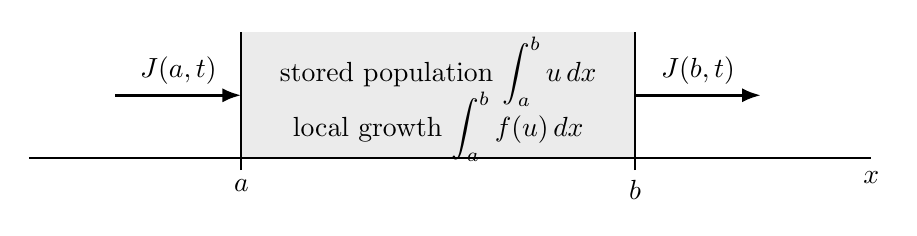
\begin{tikzpicture}[x=1cm,y=1cm,>={Latex[length=2.4mm]}]
  \fill[black!8] (3,0) rectangle (8,1.6);
  \draw[thick] (0.3,0)--(11,0);
  \draw[thick] (3,-0.15)--(3,1.6);
  \draw[thick] (8,-0.15)--(8,1.6);
  \draw[->,very thick] (1.4,0.8)--(3,0.8) node[midway,above]{$J(a,t)$};
  \draw[->,very thick] (8,0.8)--(9.6,0.8) node[midway,above]{$J(b,t)$};
  \node at (5.5,1.1) {stored population $\displaystyle\int_a^b u\,dx$};
  \node at (5.5,0.4) {local growth $\displaystyle\int_a^b f(u)\,dx$};
  \node[below] at (3,-0.15) {$a$};
  \node[below] at (8,-0.15) {$b$};
  \node[below] at (11,-0.05) {$x$};
\end{tikzpicture}
\caption{Control segment $[a,b]$. The stored population changes through the flux across the two
ends and through local growth inside the segment.}
\label{fig:controlvolume}
\end{figure}

By the fundamental theorem of calculus, $J(a,t)-J(b,t)=-\int_a^b \partial_x J\,dx$. The segment is fixed, so
the time derivative moves inside the integral, and \eqref{eq:integral} becomes
\begin{equation}
  \int_a^b\left[\pd{u}{t}+\pd{J}{x}-f(u)\right]dx=0 .
\end{equation}
This holds for \emph{every} segment $[a,b]$. If the integrand is continuous, it must vanish
everywhere: were it positive at some point, it would stay positive on a small segment around that
point and the integral would not be zero. This gives the local conservation law
\begin{equation}
  \boxed{\;\pd{u}{t}+\pd{J}{x}=f(u)\;}
  \label{eq:conservation}
\end{equation}
which is the one-dimensional form of $\partial_t u+\nabla\!\cdot\!J=f(u)$. It holds whatever the
dispersal mechanism is. The modelling lies in choosing $J$ and $f$.

\subsection{Fick's law of diffusion}
Equation~\eqref{eq:conservation} has two unknowns, so a constitutive law for the flux is needed. If
individuals move at random, more of them cross a point from the crowded side than from the sparse
side, so the net flow runs down the density gradient. Fick's law~\cite{fick} states that the
flux is proportional to that gradient:
\begin{equation}
  J=-D\,\pd{u}{x},
  \label{eq:fick}
\end{equation}
where $D>0$ is the diffusion coefficient, with units of length$^2$/time. The minus sign sends
individuals from high density to low density.

This law can also be derived from individual motion. Suppose that in each time step $\tau$ an
individual moves a distance $\ell$ left or right with equal probability. The probability $p$ of being
at $x$ then obeys $p(x,t+\tau)=\tfrac12 p(x-\ell,t)+\tfrac12 p(x+\ell,t)$. Expanding both sides in
Taylor series gives
\begin{equation}
  \tau\,\pd{p}{t}+O(\tau^2)=\frac{\ell^2}{2}\pdd{p}{x}+O(\ell^4).
\end{equation}
Dividing by $\tau$ and letting $\ell,\tau\to0$ with $D=\ell^2/(2\tau)$ held fixed gives the diffusion
equation. The coefficient $D$ therefore measures how quickly individuals wander.

\subsection{Logistic growth}
A density-independent rate $f(u)=ru$ would grow without bound. Limited resources are modelled with
the logistic law
\begin{equation}
  f(u)=r\,u\left(1-\frac{u}{K}\right),
  \label{eq:logistic}
\end{equation}
where $r>0$ is the intrinsic growth rate and $K>0$ is the carrying capacity. Figure~\ref{fig:reaction}
plots this term, scaled by $rK$. It is positive between $u=0$ and $u=K$, where the population
grows, and negative above $K$, where the population declines. The arrows show the direction of
change. The steepest growth per head occurs at very low density, where $f(u)\approx ru$; this fact
decides the wave speed in Section~\ref{sec:waves}.

\fig[0.66\textwidth]{reaction}{Logistic growth term against density. The open circle at $u=0$ is
an unstable equilibrium, and the filled circle at $u=K$ is a stable one.}

\subsection{The reaction-diffusion equation}
Substituting \eqref{eq:fick} and \eqref{eq:logistic} into \eqref{eq:conservation} with constant $D$
gives the Fisher-KPP equation:
\begin{equation}
  \boxed{\;\pd{u}{t}=D\,\pdd{u}{x}+r\,u\left(1-\frac{u}{K}\right)\;}
  \label{eq:fisher}
\end{equation}
The domain is $0\le x\le L$. The boundary condition is no flux, meaning that nobody leaves the
habitat, and the initial condition is a localized drop at the centre:
\begin{equation}
  \pd{u}{x}(0,t)=\pd{u}{x}(L,t)=0,\qquad
  u(x,0)=A\exp\!\left[-\frac{(x-L/2)^2}{2\sigma^2}\right].
  \label{eq:ibc}
\end{equation}
Integrating \eqref{eq:fisher} over the domain and using the no-flux ends gives the balance law for
the total population $M(t)=\int_0^L u\,dx$:
\begin{equation}
  \frac{dM}{dt}=\int_0^L r\,u\left(1-\frac{u}{K}\right)dx .
  \label{eq:mass}
\end{equation}
Diffusion moves individuals around but cannot change $M$. Only the reaction term can.

\subsection{Non-dimensional form}
The scalings $\tilde u=u/K$, $\tilde t=rt$ and $\tilde x=x\sqrt{r/D}$ turn \eqref{eq:fisher} into
\begin{equation}
  \pd{\tilde u}{\tilde t}=\pdd{\tilde u}{\tilde x}+\tilde u\,(1-\tilde u).
  \label{eq:nondim}
\end{equation}
All three parameters vanish, which has two consequences. First, the natural length is
$\sqrt{D/r}$ and the natural time is $1/r$, so the only speed that can be built from the
parameters is proportional to $\sqrt{rD}$. The square-root dependence of the wave speed is
already fixed by dimensional analysis, and only the factor $2$ needs a calculation. Second, it is
enough to simulate $D=r=K=1$ for the baseline, which we do unless stated otherwise.

\subsection{Pure diffusion as a limiting case}
With $r=0$, \eqref{eq:fisher} is the heat equation. On an unbounded domain, a Gaussian of variance
$\sigma_0^2$ and total mass $M$ stays Gaussian:
\begin{equation}
  u(x,t)=\frac{M}{\sqrt{2\pi(\sigma_0^2+2Dt)}}
  \exp\!\left[-\frac{(x-x_0)^2}{2(\sigma_0^2+2Dt)}\right].
  \label{eq:gaussian}
\end{equation}
The variance grows linearly as $\sigma_0^2+2Dt$, so the width grows only like $\sqrt{t}$. Diffusion
alone therefore produces \emph{no} constant-speed front: the spread slows down forever. Growth is what
converts this slowing spread into a wave of steady speed. We use \eqref{eq:gaussian} as an exact test
of the solver in Section~\ref{sec:verification}.

\subsection{Stability of the uniform states}
Uniform states satisfy $f(u)=0$, so they are $u=0$ and $u=K$. Perturbing a state $\bar u$ with
$u=\bar u+\varepsilon\,e^{ikx+\sigma t}$ and keeping terms linear in $\varepsilon$ gives
\begin{equation}
  \sigma(k)=f'(\bar u)-Dk^2 .
\end{equation}
With $f'(0)=r$ and $f'(K)=-r$, the two states behave as follows:
\begin{align}
  \bar u=0: &\quad \sigma=r-Dk^2, \quad\mbox{unstable to all modes with } k^2<r/D,\\
  \bar u=K: &\quad \sigma=-r-Dk^2<0, \quad\mbox{stable to every mode.}
\end{align}
The empty habitat is unstable and the full habitat is stable. The wave is the moving boundary along
which the stable state invades the unstable one.

% ================================================================ 3
\section{Travelling Wave Analysis}\label{sec:waves}

\subsection{Travelling wave ansatz}
The travelling-wave theory concerns an unbounded, homogeneous habitat. Our finite
no-flux domain approximates it only before the fronts interact with the boundaries.
At very long times on a finite habitat the density saturates, rather than supporting
perpetual outward propagation.
We look for solutions that keep their shape and move at constant speed $v>0$:
\begin{equation}
  u(x,t)=U(z),\qquad z=x-vt .
\end{equation}
Since $\partial_t u=-vU'$ and $\partial_{xx}u=U''$, equation \eqref{eq:fisher} reduces to an ordinary
differential equation:
\begin{equation}
  D\,U''+v\,U'+r\,U\left(1-\frac{U}{K}\right)=0 .
  \label{eq:waveode}
\end{equation}
An invasion needs $U(-\infty)=K$ behind the front, $U(+\infty)=0$ ahead of it, and $U\ge0$ throughout,
because a density cannot be negative. Writing $V=U'$ gives the first-order system
\begin{equation}
  U'=V,\qquad V'=-\frac{1}{D}\left[vV+r\,U\left(1-\frac{U}{K}\right)\right],
  \label{eq:system}
\end{equation}
with equilibria at $(0,0)$ and $(K,0)$. A wave is an orbit that connects $(K,0)$ to $(0,0)$.

\subsection{Linearisation and the minimum speed}
At the saddle $(K,0)$, linearising \eqref{eq:system} gives the characteristic equation
$D\mu^2+v\mu-r=0$, with roots
\begin{equation}
  \mu=\frac{-v\pm\sqrt{v^2+4rD}}{2D}.
\end{equation}
The roots are real with opposite signs for every $v$, so $(K,0)$ is always a saddle with exactly one
orbit leaving it into $U<K$. At $(0,0)$, the characteristic equation is $D\mu^2+v\mu+r=0$, with roots
\begin{equation}
  \mu=\frac{-v\pm\sqrt{v^2-4rD}}{2D}.
  \label{eq:originroots}
\end{equation}
If $v^2<4rD$, the roots are complex, so the origin is a stable spiral. An orbit approaching it must
wind around it and cross $U=0$, which gives negative density. No admissible wave exists. If
$v^2\ge4rD$, the roots are real and negative, the origin is a stable node, and $U$ can approach zero
without changing sign. Admissibility therefore requires
\begin{equation}
  \boxed{\;v\ge v^*=2\sqrt{rD}\;}
  \label{eq:vstar}
\end{equation}

\subsection{Existence of the wave for \texorpdfstring{$v\ge v^*$}{v >= v*}}
The linear argument shows that $v\ge v^*$ is necessary. It is also sufficient, which we show with a
trapping region. Let $m=v/(2D)$ and let $T$ be the triangle
\begin{equation}
  T=\{(U,V): 0<U<K,\ -mU<V<0\}.
\end{equation}
The orbit leaving the saddle enters $T$ at its corner $(K,0)$. No orbit can leave $T$, as each
side shows:
\begin{itemize}
  \item On the side $V=0$, $V'=-rU(1-U/K)/D<0$, so the flow points down into $T$.
  \item On the side $U=K$ with $V<0$, $U'=V<0$, so the flow points left into $T$.
  \item On the side $V=-mU$, substituting into \eqref{eq:system} and using $1-U/K\le 1$ gives
  \begin{equation}
    \frac{d}{dz}(V+mU)=\frac{U}{D}\left[vm-r\left(1-\frac{U}{K}\right)\right]-m^2U
    \;\ge\; U\left[\frac{v^2}{4D^2}-\frac{r}{D}\right]\;\ge\;0,
  \end{equation}
  where the last step uses $v^2\ge4rD$. Hence $V+mU$ cannot decrease here, and the flow does not cross this side.
\end{itemize}
Inside $T$, $U'=V<0$, so $U$ decreases monotonically along the orbit, and the orbit can only end at
$(0,0)$. A monotone wave with $0<U<K$ thus exists for every $v\ge v^*$. Figure~\ref{fig:phase_plane}
shows this numerically. Each panel draws the direction field of \eqref{eq:system} with the orbit
leaving $(K,0)$, computed with $D=r=K=1$. At $v=1$ the orbit overshoots into $U<0$ and spirals, so it is
not a population. At $v=2$ it arrives at the origin without crossing into negative density.

\fig{phase_plane}{Phase plane of the travelling wave system for a speed below $v^*$ (left) and at
$v^*$ (right). The filled circle is the saddle $(K,0)$ and the open circle is the origin.}

\subsection{Why the slowest wave is selected}
Equation~\eqref{eq:vstar} gives a whole family of speeds, so we need to know which one a real drop
selects. The answer comes from the leading edge. Far ahead of the front, $u\ll K$, so the logistic
term is nearly linear and the equation becomes $\partial_t u=D\partial_{xx}u+ru$. Substituting an
exponential edge $u\sim e^{-\lambda(x-vt)}$ gives the dispersion relation
\begin{equation}
  v(\lambda)=D\lambda+\frac{r}{\lambda},
  \label{eq:dispersion}
\end{equation}
plotted in Figure~\ref{fig:dispersion}. Setting $dv/d\lambda=D-r/\lambda^2=0$ gives the minimum at
\begin{equation}
  \lambda^*=\sqrt{\frac{r}{D}},\qquad v(\lambda^*)=2\sqrt{rD}=v^* .
  \label{eq:lambdastar}
\end{equation}

\fig[0.66\textwidth]{dispersion}{Speed of an exponential leading edge against its decay rate, in
scaled units. Every speed above $v^*$ corresponds to two decay rates. Compact initial data selects the
minimum.}

Equation~\eqref{eq:dispersion} carries a striking physical message: neither $K$ nor the
nonlinearity appears. The front is \emph{pulled} by the sparse individuals at its tip, who
reproduce at the full rate $r$ and wander with coefficient $D$~\cite{saarloos}. The bulk of the
population behind them only follows. The selection rule for initial data decaying like
$e^{-\lambda|x|}$ is~\cite{bramson,saarloos}
\begin{equation}
  v_{\mbox{selected}}=
  \begin{cases}
    D\lambda+r/\lambda, & \lambda<\lambda^*,\\
    2\sqrt{rD}, & \lambda\ge\lambda^*.
  \end{cases}
  \label{eq:selection}
\end{equation}
The Gaussian drop used here has a tail that falls off faster than any exponential, so it lies in the second case
and spreads at $v^*$, as proved by Kolmogorov, Petrovsky and Piskunov~\cite{kpp} and extended by
Aronson and Weinberger~\cite{aronson}. At $v=v^*$, the two roots in \eqref{eq:originroots} coincide,
so the far field takes the form $U\sim(Az+B)\,e^{-\lambda^* z}$.

\subsection{The approach to the asymptotic speed}
The speed $v^*$ is only reached as $t\to\infty$, and it is approached slowly. Bramson~\cite{bramson}
proved that the front position from compact initial data obeys
\begin{equation}
  X(t)=2\sqrt{rD}\;t-\frac32\sqrt{\frac{D}{r}}\,\ln(rt)+O(1).
  \label{eq:bramson}
\end{equation}
The leading asymptotic relaxation of the instantaneous speed is
$v^*-\tfrac32\sqrt{D/r}\,/t$. This uses refined front-asymptotic theory~\cite{saarloos};
it does not follow simply by differentiating an unspecified $O(1)$ remainder.
The corresponding leading prediction for the endpoint-average speed over $[t_1,t_2]$ is
\begin{equation}
  \bar v\approx v^*-\frac32\sqrt{\frac{D}{r}}\;\frac{\ln(t_2/t_1)}{t_2-t_1}.
  \label{eq:meanspeed}
\end{equation}
This correction applies at late times on an effectively unbounded habitat, before boundary
effects arise. It predicts a speed below $v^*$ for our steep initial drop. A least-squares slope
and an endpoint-average speed use different weights, so equation~\eqref{eq:meanspeed} is used
as an approximation when comparing with fitted slopes. It is not an exact finite-time identity.

\subsection{An exact solution}
For the special speed $v=5\sqrt{rD/6}\approx2.04\sqrt{rD}$, equation~\eqref{eq:fisher} has the closed-form
solution of Ablowitz and Zeppetella~\cite{ablowitz}:
\begin{equation}
  u(x,t)=K\left[1+C\exp\!\left(\sqrt{\frac{r}{6D}}\;\Big(x-5\sqrt{\frac{rD}{6}}\,t\Big)\right)\right]^{-2}.
  \label{eq:exact}
\end{equation}
This is one member of the wave family above $v^*$. It provides an exact benchmark for measuring the
order of accuracy of the solver.

% ================================================================ 4
\section{Numerical Method}\label{sec:numerics}

\subsection{Grid and finite differences}
The discretisation below follows standard finite difference practice~\cite{leveque}.
The domain $[0,L]$ is divided into $N$ intervals of width $\Delta x=L/N$, with nodes $x_i=i\Delta x$.
Time advances in steps of $\Delta t$, with $t^n=n\Delta t$ and $u_i^n\approx u(x_i,t^n)$.
Adding the Taylor expansions of $u(x\pm\Delta x,t)$ cancels the odd derivatives and gives the
central difference
\begin{equation}
  \pdd{u}{x}\bigg|_i=\frac{u_{i+1}-2u_i+u_{i-1}}{\Delta x^2}-\frac{\Delta x^2}{12}\,\frac{\partial^4u}{\partial x^4}\bigg|_i+O(\Delta x^4).
\end{equation}
Likewise, the forward Euler difference in time is
\begin{equation}
  \pd{u}{t}\bigg|^n=\frac{u^{n+1}-u^n}{\Delta t}-\frac{\Delta t}{2}\,\pdd{u}{t}\bigg|^n+O(\Delta t^2).
\end{equation}

\subsection{The explicit update}
Substituting these differences into \eqref{eq:fisher} and solving for the new value gives
\begin{equation}
  \boxed{\;u_i^{n+1}=u_i^n+\alpha\left(u_{i+1}^n-2u_i^n+u_{i-1}^n\right)
  +\Delta t\,r\,u_i^n\left(1-\frac{u_i^n}{K}\right)\;},
  \qquad \alpha=\frac{D\,\Delta t}{\Delta x^2}.
  \label{eq:ftcs}
\end{equation}
Figure~\ref{fig:stencil} shows the stencil: each new value depends on three old values. The scheme is
explicit, so no system of equations needs solving, and the local truncation error is
$O(\Delta t)+O(\Delta x^2)$.

\begin{figure}[H]
\centering
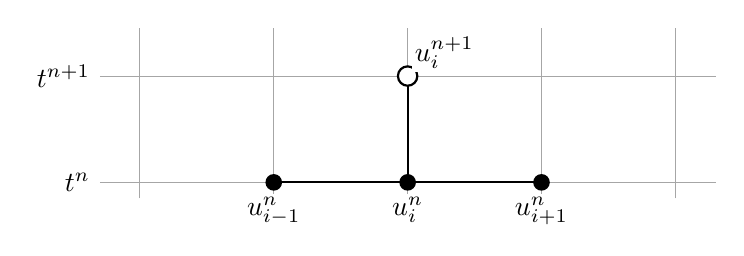
\begin{tikzpicture}[x=1.7cm,y=1.35cm]
  \foreach \x in {0,1,2,3,4}{\draw[black!35] (\x,-0.15)--(\x,1.45);}
  \foreach \y in {0,1}{\draw[black!35] (-0.3,\y)--(4.3,\y);}
  \draw[thick] (1,0)--(3,0);
  \draw[thick] (2,0)--(2,1);
  \foreach \x in {1,2,3}{\fill[black] (\x,0) circle (3pt);}
  \filldraw[fill=white,draw=black,thick] (2,1) circle (3.5pt);
  \node[below=4pt,fill=white,inner sep=1pt] at (1,0) {$u_{i-1}^n$};
  \node[below=4pt,fill=white,inner sep=1pt] at (2,0) {$u_{i}^n$};
  \node[below=4pt,fill=white,inner sep=1pt] at (3,0) {$u_{i+1}^n$};
  \node[above right=2pt,fill=white,inner sep=1pt] at (2,1) {$u_{i}^{n+1}$};
  \node[left] at (-0.3,0) {$t^n$};
  \node[left] at (-0.3,1) {$t^{n+1}$};
\end{tikzpicture}
\caption{Stencil of the explicit scheme. The new value (open circle) is computed from three known
values at the previous time level (filled circles).}
\label{fig:stencil}
\end{figure}

\subsection{No-flux boundaries and discrete mass}
The no-flux condition is imposed with a mirror ghost node, $u_{-1}=u_1$, which makes the centred
difference of $\partial_x u$ vanish at $x=0$ and keeps second-order accuracy. The end update becomes
\begin{equation}
  u_0^{n+1}=u_0^n+2\alpha\left(u_1^n-u_0^n\right)+\Delta t\,r\,u_0^n\left(1-\frac{u_0^n}{K}\right),
\end{equation}
and likewise at $x=L$. With this choice, the scheme conserves population exactly when $r=0$. Let
$M^n=\Delta x\left(\tfrac12u_0^n+\sum_{i=1}^{N-1}u_i^n+\tfrac12u_N^n\right)$ be the trapezoidal mass.
Then, using the telescoping of the interior sum,
\begin{equation}
  \frac{M^{n+1}-M^n}{\alpha\,\Delta x}
  =(u_1-u_0)+\sum_{i=1}^{N-1}(u_{i+1}-2u_i+u_{i-1})+(u_{N-1}-u_N)=0 .
\end{equation}
This is the discrete form of the statement that diffusion cannot change the total population in
\eqref{eq:mass}, and it provides a sharp test of the code.

\subsection{Stability}\label{sec:stability}
\subsubsection{Von Neumann analysis}
We linearise \eqref{eq:ftcs} about a uniform state $\bar u$ and insert the Fourier mode
$\varepsilon_i^n=\xi^n e^{\mathrm{i}ki\Delta x}$. Using $e^{\mathrm{i}\theta}+e^{-\mathrm{i}\theta}-2=-4\sin^2(\theta/2)$, the amplification
factor is
\begin{equation}
  \xi=1+\Delta t\,f'(\bar u)-4\alpha\sin^2\!\left(\frac{k\Delta x}{2}\right).
\end{equation}
For $r=0$, this yields the classical diffusion limit $\alpha\le\tfrac12$, that is,
$\Delta t\le\Delta x^2/(2D)$. With growth included, the critical state is the plateau $\bar u=K$, where
$f'=-r$. At the grid-scale mode $k\Delta x=\pi$, $\xi=1-r\Delta t-4\alpha$, and $\xi\ge-1$ requires
\begin{equation}
  \Delta t\le\frac{2}{4D/\Delta x^2+r}.
  \label{eq:vonneumann}
\end{equation}
This is \emph{stricter} than the diffusion limit: the reaction term lowers the safe time step.

\subsubsection{A maximum principle}
Stability in the von Neumann sense does not guarantee that the density stays physical. We prove a
stronger result. Write \eqref{eq:ftcs} as
\begin{equation}
  u_i^{n+1}=\alpha u_{i+1}^n+\alpha u_{i-1}^n+g(u_i^n),\qquad
  g(s)=(1-2\alpha)s+\Delta t\,r\,s\left(1-\frac{s}{K}\right).
\end{equation}
On $0\le s\le K$, $g'(s)=1-2\alpha+r\Delta t(1-2s/K)\ge1-2\alpha-r\Delta t$. Suppose that
\begin{equation}
  \boxed{\;\Delta t\le\frac{1}{2D/\Delta x^2+r}\;}
  \label{eq:monotone}
\end{equation}
Then $g'\ge0$, so $g$ is non-decreasing on $[0,K]$. If $0\le u_i^n\le K$ for all $i$, then
\begin{align}
  u_i^{n+1}&\ge 0+0+g(0)=0,\\
  u_i^{n+1}&\le \alpha K+\alpha K+g(K)=2\alpha K+(1-2\alpha)K=K .
\end{align}
By induction, the density remains within $[0,K]$ for all time. This establishes an invariant interval and an order-preserving update; it does not rule out all temporal variation.
The mirror-node updates at the ends have the same form. The solver refuses any larger step unless
told otherwise. If $K$ varies in space, the same argument on $[0,K_{\max}]$ gives
\begin{equation}
  \Delta t\le\frac{1}{2D/\Delta x^2+r\,(2K_{\max}/K_{\min}-1)}.
  \label{eq:monotonevar}
\end{equation}

\subsection{The wave speed of the scheme itself}\label{sec:discretespeed}
The discrete equations have their own front speed, which we can compute exactly. Substituting
$u_i^n=e^{-\lambda(x_i-vt^n)}$ into \eqref{eq:ftcs} linearised about $u=0$ gives
$e^{\lambda v\Delta t}=1+r\Delta t+2\alpha\left(\cosh\lambda\Delta x-1\right)$, so
\begin{equation}
  v_h(\lambda)=\frac{1}{\lambda\Delta t}\ln\!\left[1+r\Delta t+2\alpha\left(\cosh\lambda\Delta x-1\right)\right].
  \label{eq:vh}
\end{equation}
As for \eqref{eq:dispersion}, the scheme selects the minimum, $v_h=\min_\lambda v_h(\lambda)$. Expanding
\eqref{eq:vh} for small steps around $\lambda^*$ with $D=r=1$ gives
\begin{equation}
  v_h\approx 2+\frac{\Delta x^2}{12}-2\Delta t ,
  \label{eq:vhapprox}
\end{equation}
with higher-order terms $O(\Delta x^4+\Delta x^2\Delta t+\Delta t^2)$. Thus the leading spatial and temporal errors have opposite signs. The Euler step slows the front,
and the central difference speeds it up. Equation~\eqref{eq:vh} replaces $v^*$ as the correct target
for a simulation on a finite grid.

\subsection{Algorithm}
Algorithm~\ref{alg:ftcs} is the method as implemented in \code{solve\_loops}. The spatial loop
is nested inside the temporal loop, as the problem statement requires. The full source is in Appendix~\ref{app:code} and the linked repository.

\begin{algorithm}[H]
\caption{Explicit finite difference solver for the Fisher-KPP equation}
\label{alg:ftcs}
\KwIn{$D,r,K$; grid $x_0,\dots,x_N$; initial density $u^0$; step $\Delta t$; final time $T$}
\KwOut{Density snapshots}
$\alpha\leftarrow D\Delta t/\Delta x^2$\;
Check that $\Delta t$ satisfies the bound \eqref{eq:monotone}\;
\For(\tcp*[f]{temporal Euler loop}){$n=0$ \KwTo $T/\Delta t-1$}{
  \For(\tcp*[f]{spatial second-derivative loop}){$i=1$ \KwTo $N-1$}{
    $u_{xx}\leftarrow(u_{i+1}-2u_i+u_{i-1})/\Delta x^2$\;
    $u_i^{\mbox{new}}\leftarrow u_i+\Delta t\left[Du_{xx}+ru_i(1-u_i/K)\right]$\;
  }
  Update $u_0^{\mbox{new}}$ and $u_N^{\mbox{new}}$ using the mirror ghost nodes\;
  Swap $u$ and $u^{\mbox{new}}$\;
  Save a snapshot at the chosen interval\;
}
\end{algorithm}

If $T/\Delta t$ is not an integer, the implementation shortens the last Euler step
to end exactly at $T$. It always saves the final state, even if that time is not on
the regular snapshot cadence. Both solver engines validate that the grid is uniform.

\subsection{Measuring the front}
The front position $X(t)$ is the point where the density crosses a fixed level, by default $K/2$. On
each snapshot the code finds the outermost node at or above the level and locates the crossing
by linear interpolation between nodes, so that $X(t)$ is not locked to the grid. The speed is the
slope of a least-squares line through $X(t)$ over a chosen time window, reported with its standard error.

% ================================================================ 5
\clearpage
\section{Procedure}\label{sec:procedure}

\subsection{Code organisation}
The complete programming code is printed in Appendix~\ref{app:code}. Runnable source,
generated figures, numerical data and animations are available in the project repository:
\begin{center}\small
\url{https://github.com/awmbw/Reaction-Diffusion-Population-Dispersal}
\end{center}
The repository contains \code{rdpop/}, \code{tests/}, \code{outputs/}, and the editable
LaTeX source in \code{report/}. The final PDF is in \code{submission/}.
Direct links are provided to the
\href{https://github.com/awmbw/Reaction-Diffusion-Population-Dispersal/tree/main/outputs/figures}{generated figures},
\href{https://github.com/awmbw/Reaction-Diffusion-Population-Dispersal/blob/main/outputs/animations/wave_spreading.gif}{spreading-wave animation}, and
\href{https://github.com/awmbw/Reaction-Diffusion-Population-Dispersal/blob/main/outputs/animations/capacity_gradient.gif}{capacity-gradient animation}.
The code is a small Python package, \code{rdpop}, and its modules are listed in
Table~\ref{tab:modules}. Pure Python loops are slow, so \code{solver.py} holds two engines with the same
interface: \code{solve\_loops}, the reference solver with explicit nested loops, and \code{solve\_vector},
which applies the same update with NumPy array slices. The main experiment uses the nested
loops. Long runs and parameter sweeps use the array engine.

\begin{table}[H]
\centering\small
\caption{Modules of the code base.}
\label{tab:modules}
\begin{tabularx}{\textwidth}{lL}
\toprule
File & Purpose\\
\midrule
\code{rdpop/solver.py} & Grid, stability limit, and the two solver engines\\
\code{rdpop/theory.py} & Closed-form results: speeds, exact solutions, wave orbit\\
\code{rdpop/analysis.py} & Front tracking, line fits, mass and error norms\\
\code{rdpop/experiments.py} & All numerical experiments and their parameters\\
\code{rdpop/figures.py} & All figures in this report\\
\code{rdpop/animations.py} & Animated line plots, written as GIF files\\
\code{rdpop/report\_data.py} & Writes measured values into the report as LaTeX macros\\
\code{run\_all.py} & Runs the whole pipeline\\
\code{tests/test\_rdpop.py} & Automated checks of the solver, theory and analysis\\
\bottomrule
\end{tabularx}
\end{table}

\subsection{Steps to reproduce the results}
\begin{enumerate}
    \item Download or clone the repository above, then work from its root.
        Install Python 3.10 or later, create a virtual environment, and install the dependencies:
        \code{pip install -r requirements.txt}.
  \item Run the automated checks from the repository root: \code{python -m pytest tests}.
  \item Generate every result: \code{python run\_all.py}.
  \item Find the figures in \code{outputs/figures}, the animations in \code{outputs/animations}, and the
        measured values in \code{outputs/data}.
  \item Rebuild the report with \code{make report} or follow the compiler instructions
        in the repository README.
\end{enumerate}

Measured summary values and result tables are written by \code{report\_data.py} from the
simulation output and read by the LaTeX source.

\subsection{Baseline parameters}
Table~\ref{tab:params} lists the baseline values. They are scaled units, following
\eqref{eq:nondim}, so a result can be converted to any real species by supplying its $D$, $r$ and $K$.
The ratio $\alpha=$~\resBaseAlpha{} is chosen well inside the limit: the bound \eqref{eq:monotone} allows
$\Delta t\le$~\resBaseDtLimit{}. Small steps are used here because Section~\ref{sec:discretespeed} shows that
the time step directly biases the front speed.

\begin{table}[H]
\centering\small
\caption{Baseline parameters, in scaled units.}
\label{tab:params}
\begin{tabular}{lcc}
\toprule
Quantity & Symbol & Value\\
\midrule
Diffusion coefficient & $D$ & 1\\
Growth rate & $r$ & 1\\
Carrying capacity & $K$ & 1\\
Domain length & $L$ & 200\\
Drop amplitude and width & $A$, $\sigma$ & 0.5, 1\\
Grid spacing & $\Delta x$ & 0.2\\
Time step & $\Delta t$ & 0.0025\\
Final time & $T$ & 40\\
\bottomrule
\end{tabular}
\end{table}

% ================================================================ 6
\section{Results: The Spreading Population Wave}\label{sec:results}

\subsection{Spreading of a central drop}
Figure~\ref{fig:snapshots} shows the density at six times, from the nested-loop solver. These are
frames of the animation \code{outputs/animations/wave\_spreading.gif}, which shows the same motion
continuously. At first, the drop grows in place while diffusion rounds it. By $t=5$, it has nearly
reached the carrying capacity at its centre and has started to widen. By $t=10$, a flat plateau at
$u=K$ has formed, bounded by two steep fronts, and from then on the fronts keep their shape and
their spacing widens evenly. This is the behaviour Section~\ref{sec:waves} predicts: the habitat
fills up behind two outward-moving waves. Since $L$ was chosen large enough, neither front has
reached a boundary by $t=40$.

\fig{snapshots}{Population density at six times after a central drop. Darker curves are later times.
Two fronts of fixed shape move outward, leaving the habitat at carrying capacity.}

\subsection{Spatiotemporal heatmap}
Figure~\ref{fig:heatmap} shows the same run as a heatmap, with time on the vertical axis, space on
the horizontal axis and density as colour. The whole history is visible at once. White regions are
empty, dark regions are full, and the narrow band between them is the front. The V shape has straight
edges, which is the visual signature of a constant speed, since a pure diffusion spread would instead
trace a curve $|x-L/2|\propto\sqrt{t}$. The dashed guides represent front speeds
$dx/dt=\pm v^*=\pm2$, so their plotted slopes are $dt/dx=\pm1/2$ with these axes.
They pass through the measured fronts at $t=40$ and track them closely over most of the run. The small
separation at early times is the slow approach to $v^*$ analysed below.

\fig{heatmap}{Spatiotemporal heatmap of density, with time on the Y axis and space on the X axis.
Dashed guides represent the theoretical front speed $v^*=2$; their plotted slopes are $dt/dx=\pm1/2$.}

\subsection{Measured wave speed}
The left panel of Figure~\ref{fig:front} plots the distance of each front from the centre. The curves
for the right and left fronts lie on top of each other, as symmetry requires: the fitted speeds are
\resBaseSpeed{} and \resLeftSpeed{}. The straight-line fit over $20\le t\le40$ gives
\begin{center}
  $v_{\mathrm{measured}}=$ \resBaseSpeed{} $\pm$ \resBaseSpeedErr{}, \qquad $R^2=$ \resBaseRsq{}.
\end{center}
The result is close to, but clearly below, the theoretical $v^*=2$, by \resBasePercentLow{}\,\%. The quoted standard error describes residual scatter about a straight line. These deterministic
samples are correlated, so it is not a confidence bound on the physical speed and excludes
discretisation and finite-time bias. We therefore compare the result with theory and refinement studies.

\fig{front}{Left: distance of each front from the centre, with the straight-line fit. Right: front
speed over a long run on a logarithmic time axis, with the prediction from the Bramson correction.}

Two known effects account for the gap. Equation~\eqref{eq:vh} gives the scheme's own speed, $v_h=$
\resGridSpeed{} for these grid values. Equation~\eqref{eq:meanspeed} gives the Bramson delay
over the window $[20,40]$, a reduction of \resBaseDelay{}. Together they predict
\begin{center}
  $v_{\mathrm{predicted}}=$ \resGridSpeed{} $-$ \resBaseDelay{} $=$ \resBasePredicted{},
\end{center}
which differs from the measurement by \resBaseGap{}. This supports the leading finite-time
explanation. The comparison combines a discrete speed with a continuum delay coefficient;
the discrete leading-edge decay rate and higher-order relaxation introduce additional corrections. The right panel of Figure~\ref{fig:front}
confirms this. It plots the measured speed from a long run, computed on a domain large enough to
hold the front until $t=160$. The speed rises towards $v^*$ and follows the curve $v_h-3/(2t)$ closely
at late times.

Table~\ref{tab:windows} makes the same comparison for four time windows. Each doubling of the
time window halves the delay, and the measured slopes follow the prediction. The largest
difference is in the earliest window, as expected, because \eqref{eq:bramson} holds for large $t$.

\begin{table}[H]
\centering\small
\caption{Measured front speed in four time windows, compared with the corrected prediction.}
\label{tab:windows}
\begin{tabular}{ccccc}
\toprule
Window & Measured slope & Delay & Predicted $v_h-{}$delay & Difference \\
\midrule
$[10,20]$ & 1.8883 & 0.1040 & 1.8944 & -0.0060 \\
$[20,40]$ & 1.9473 & 0.0520 & 1.9463 & +0.0009 \\
$[40,80]$ & 1.9739 & 0.0260 & 1.9723 & +0.0016 \\
$[80,160]$ & 1.9863 & 0.0130 & 1.9853 & +0.0010 \\
\bottomrule
\end{tabular}

\end{table}

A direct test of \eqref{eq:bramson} is to fit $X(t)=vt-c\ln t+b$ to the long run for $t\ge20$. This gives
$v=$~\resLongSpeed{} and $c=$~\resLongDelay{}, against the predictions $v_h=$~\resLongGrid{} and $c=3/2$. The
speed agrees to \resLongGap{}\,\%. The fitted logarithmic coefficient is consistent
with $3/2$ at this resolution and time range; it is an empirical consistency check.

The speed does not depend materially on the level used to define the front. Measured at
$u=0.1$, $0.5$ and $0.9$, it is \resSpeedTen{}, \resSpeedFifty{} and \resSpeedNinety{}. The lower level moves slightly
faster, so the front is still slowly broadening towards its final shape, which is itself a
finite-time effect.

\subsection{Shape of the wave}
Figure~\ref{fig:profile} checks that the front really is the travelling wave of
Section~\ref{sec:waves}. In the left panel, profiles at three late times are shifted by their front
positions, and the curves collapse onto one shape. The dashed curve is obtained independently
by integrating the wave ODE \eqref{eq:waveode} at $v=2$. The largest difference between it and
the final profile is \resProfileGap{} for $-10<z<8$, so the PDE and the ODE give the same wave.

The right panel uses a logarithmic density axis to expose the leading edge. Here the profile is
a straight line over many decades, and its slope matches the predicted exponential
$e^{-\lambda^*z}$ with $\lambda^*=1$. Fitting the form $Az\,e^{-\lambda z}$ gives
$\lambda=$~\resEdgeDecay{}. This is the region that pulls the front, and the agreement over many orders of
magnitude supports the pulled-front picture.

\fig{profile}{Left: late-time profiles in the frame of the front, with the wave from the ODE (dashed).
Right: the same profiles on a logarithmic axis, showing the exponential leading edge.}

\subsection{Total population}
Equation~\eqref{eq:mass} says that, once the fronts have formed, the population grows only by
adding new area at the two fronts. Each front adds $vK$ per unit time, so $dM/dt\to2vK$.
Figure~\ref{fig:mass} shows that $M(t)$ indeed becomes a straight line. The fitted slope is
\resMassSlope{}, and twice the predicted front speed is \resMassPredicted{}. This is very different from the
isolated logistic model, where $M$ saturates. In the spatial model, the population keeps growing
linearly until the fronts reach the boundary.

\fig[0.66\textwidth]{mass}{Total population against time. After a short transient, the population grows
linearly at twice the front speed.}

\subsection{The square-root law}
To test how the speed depends on the parameters, we simulated sixteen combinations of $r$ and $D$, each
with the same fixed mesh. Figure~\ref{fig:sweep} compares the results with \eqref{eq:vstar} on
logarithmic axes. The open squares are the raw fitted slopes, which lie just under the theory line.
The filled circles add back the Bramson delay for each case, and they fall on the line. A
power-law fit of the corrected speeds to $v=C(rD)^p$ gives
$p=$~\resSweepExponent{} and $C=$~\resSweepPrefactor{}, matching the theoretical $p=1/2$ and $C=2$. The
largest relative error is \resSweepMaxError{}\,\% (Table~\ref{tab:sweep}), and it occurs for the
smallest $D$ and largest $r$, where the fixed mesh resolves the front least well.

\fig[0.6\textwidth]{sweep}{Simulated front speed against $2\sqrt{rD}$ for sixteen parameter pairs.
Pairs with the same product $rD$ share a position on the horizontal axis.}

\begin{table}[H]
\centering\small
\caption{Front speed for each parameter pair. ``Corrected'' adds the Bramson delay to the measured slope.}
\label{tab:sweep}
\begin{tabular}{cccccc}
\toprule
$r$ & $D$ & $2\sqrt{rD}$ & Measured & Corrected & Error (\%) \\
\midrule
0.25 & 0.25 & 0.5000 & 0.4866 & 0.4996 & -0.08 \\
0.25 & 0.5 & 0.7071 & 0.6886 & 0.7069 & -0.02 \\
0.25 & 1 & 1.0000 & 0.9744 & 1.0004 & +0.04 \\
0.25 & 2 & 1.4142 & 1.3785 & 1.4152 & +0.07 \\
0.5 & 0.25 & 0.7071 & 0.6876 & 0.7060 & -0.16 \\
0.5 & 0.5 & 1.0000 & 0.9732 & 0.9992 & -0.08 \\
0.5 & 1 & 1.4142 & 1.3771 & 1.4139 & -0.02 \\
0.5 & 2 & 2.0000 & 1.9489 & 2.0009 & +0.04 \\
1 & 0.25 & 1.0000 & 0.9711 & 0.9971 & -0.29 \\
1 & 0.5 & 1.4142 & 1.3752 & 1.4119 & -0.16 \\
1 & 1 & 2.0000 & 1.9465 & 1.9985 & -0.08 \\
1 & 2 & 2.8284 & 2.7542 & 2.8277 & -0.02 \\
2 & 0.25 & 1.4142 & 1.3700 & 1.4068 & -0.53 \\
2 & 0.5 & 2.0000 & 1.9422 & 1.9942 & -0.29 \\
2 & 1 & 2.8284 & 2.7503 & 2.8239 & -0.16 \\
2 & 2 & 4.0000 & 3.8930 & 3.9970 & -0.08 \\
\bottomrule
\end{tabular}

\end{table}

\subsection{Speed selection by the initial condition}
Equation~\eqref{eq:selection} predicts that a slowly decaying initial tail overrides $v^*$. We tested this
with initial data decaying like $e^{-\lambda|x|}$ for seven values of $\lambda$. Figure~\ref{fig:selection} and
Table~\ref{tab:selection} show the results. For $\lambda<1$, the speed follows
$v=\lambda+1/\lambda$, reaching more than twice $v^*$ at $\lambda=0.25$. Above $\lambda=1$, the speed stops
depending on the initial data and approaches $v^*$. The tail sets the speed because the front is pulled
from its tip. For $\lambda>1$, the small speed deficit is consistent with steep-tail relaxation.
The marginal tail $\lambda=1$ has a different leading logarithmic shift,
$X(t)=2t-\tfrac12\ln t+O(1)$ in scaled units~\cite{saarloos}, so the $3/2$ coefficient
for steep data does not apply to that case. This experiment shows why $2\sqrt{rD}$ is the speed of a \emph{localized} drop specifically.

\fig[0.66\textwidth]{selection}{Front speed against the decay rate of the initial tail, with the
selection rule \eqref{eq:selection}.}

\begin{table}[H]
\centering\small
\caption{Selected speed for each initial decay rate.}
\label{tab:selection}
\begin{tabular}{ccc}
\toprule
$\lambda$ & Theory & Measured \\
\midrule
0.25 & 4.2500 & 4.2444 \\
0.4 & 2.9000 & 2.8960 \\
0.6 & 2.2667 & 2.2635 \\
0.8 & 2.0500 & 2.0462 \\
1 & 2.0000 & 1.9800 \\
1.5 & 2.0000 & 1.9546 \\
2 & 2.0000 & 1.9522 \\
\bottomrule
\end{tabular}

\end{table}

% ================================================================ 7
\section{Verification of the Solver}\label{sec:verification}

The agreement above is meaningful only if the solver itself is correct. This section tests it against
results that are known exactly. The file \code{tests/test\_rdpop.py} runs these checks automatically.

\subsection{Agreement of the two engines}
For the baseline, the nested-loop solver performs about \resBaseUpdates{} million point updates in
\resLoopSeconds{}\,s, and the array engine takes \resVectorSeconds{}\,s, about \resSpeedUp{} times faster.
These timings are from one run on one machine and only indicate the scale of the difference. The
largest difference between their results over the whole run is \resEngineDiff{}, so the two engines are
interchangeable and the sweeps with the fast engine are as valid as the nested-loop solver.

\subsection{Pure diffusion}
With $r=0$, the exact solution \eqref{eq:gaussian} is available. The left panel of
Figure~\ref{fig:diffusion} overlays it on the numerical solution at three times, and the two
cannot be told apart: the largest difference at $t=40$ is \resGaussError{}. The right panel shows that
the variance grows linearly at the rate $2D$; the fitted slope is \resVarianceSlope{}. The largest
relative drift in total mass over the run is \resMassDrift{}, which is round-off, as the
discrete conservation proof in Section~\ref{sec:numerics} requires.

\fig{diffusion}{Pure diffusion test. Left: numerical profiles and the exact Gaussian. Right: growth of the
variance, compared with the exact result.}

\subsection{Order of accuracy}
Equation~\eqref{eq:exact} gives an exact nonlinear solution. We started from it at $t=0$, imposed its
exact values at both ends, and measured the error at $t=5$. For the spatial study, $\Delta x$ was halved
with $\alpha=0.25$ held fixed, so that $\Delta t\propto\Delta x^2$ and the total error scales as $\Delta x^2$.
For the temporal study, $\Delta x=0.1$ was held fixed, and each run was compared with a run using a
much smaller step on the same grid, so that the spatial error cancels. Figure~\ref{fig:convergence}
shows the results. Coupled refinement gives an observed order of \resSpaceOrder{} as a function
of $\Delta x$, consistent with $O(\Delta t)+O(\Delta x^2)=O(\Delta x^2)$ when
$\Delta t\propto\Delta x^2$. This measures the combined space-time error, rather than
isolating the spatial error alone. The temporal study gives order \resTimeOrder{} on a fixed
grid. Table~\ref{tab:space} lists the errors under coupled refinement.

\fig{convergence}{Error against step size on logarithmic axes. Left: coupled refinement with
$\Delta t\propto\Delta x^2$, compared with the exact wave. Right: temporal refinement on a fixed grid
against a fine-step reference. The dotted lines show the theoretical
orders.}

\begin{table}[H]
\centering\small
\caption{Coupled space-time refinement against the exact solution at $t=5$, with $\Delta t\propto\Delta x^2$.}
\label{tab:space}
\begin{tabular}{cccc}
\toprule
$\Delta x$ & $\Delta t$ & $L^2$ error & $L^\infty$ error \\
\midrule
0.5 & $6.2\times 10^{-2}$ & $7.0\times 10^{-2}$ & $3.2\times 10^{-2}$ \\
0.25 & $1.6\times 10^{-2}$ & $1.8\times 10^{-2}$ & $8.3\times 10^{-3}$ \\
0.125 & $3.9\times 10^{-3}$ & $4.5\times 10^{-3}$ & $2.1\times 10^{-3}$ \\
0.0625 & $9.8\times 10^{-4}$ & $1.1\times 10^{-3}$ & $5.2\times 10^{-4}$ \\
\bottomrule
\end{tabular}

\end{table}

\subsection{Stability limits}
For $\Delta x=0.5$ and $D=r=1$, the three limits from Section~\ref{sec:stability} are distinct: the
maximum-principle bound \eqref{eq:monotone} is \resMonotoneLimit{}, the von Neumann bound
\eqref{eq:vonneumann} is \resVonNeumannLimit{}, and the classical diffusion limit is \resDiffusionLimit{}.
Figure~\ref{fig:stability} tests them with three runs. The sawtooth amplitude in the right panel measures
the grid-scale content $\max_i|u_{i+1}-2u_i+u_{i-1}|/4$.

Below both reaction-aware bounds, at $\Delta t=0.1$, the solution is smooth. At $\Delta t=$~\resStableDt{}, the
step exceeds the monotone bound but not the von Neumann bound, and the run remains stable. The
step $\Delta t=0.125$ gives $\alpha=0.5$, exactly the classical limit, which a diffusion analysis would call
safe. It is not. A sawtooth grows from the plateau, as shown in the left panel, and the run overflows
at $t\approx$~\resBlowUp{}. The growth starts on the plateau rather than at the fronts, as predicted,
because $\bar u=K$ is the state where $f'=-r$. This confirms that \eqref{eq:vonneumann}, and not the
classical limit, is the correct stability condition for this equation.

\fig{stability}{Runs on either side of the stability limits. Left: density shortly before the unstable
run fails. Right: sawtooth amplitude against time. The two stable curves fall after $t\approx 28$, when
the fronts reach the boundaries.}

\subsection{Discrete wave speed}
Figure~\ref{fig:discrete} tests \eqref{eq:vh}. Each point is a simulated front speed with the Bramson
delay added back, and each curve is the discrete theory, which has no fitted parameters. In the left panel,
$\Delta x$ varies with $\alpha=0.25$ held fixed. In the right panel, $\Delta t$ varies on a fixed grid. The
points follow the curves in both panels, including at the coarse grid $\Delta x=0.8$, where the speed
is more than 10\,\% below $v^*$. The right panel shows the systematic slowing of the front as
$\Delta t$ grows, as \eqref{eq:vhapprox} predicts. This also gives a practical rule: a front speed
accurate to within $\epsilon$ requires roughly $\Delta t<\epsilon/2$ and $\Delta x<\sqrt{12\epsilon}$ in scaled
units, a useful leading-order guideline. To allocate a combined absolute speed-error budget
$\epsilon$ without relying on cancellation, assign $\epsilon/2$ to each leading term:
$\Delta t\lesssim\epsilon/4$ and $\Delta x\lesssim\sqrt{6\epsilon}$.
Finite-time relaxation and boundary effects must also be controlled.

\fig{discrete}{Front speed of the numerical scheme. The curves are the exact discrete theory and the points
are simulation results. Left: varying the grid. Right: varying the time step.}

% ================================================================ 8
\section{Extension: A Spatially Varying Environment}\label{sec:extension}

\subsection{Model}
So far the habitat has been uniform. We now make the carrying capacity depend on position, with
a favourable centre and poor edges:
\begin{equation}
  \pd{u}{t}=D\pdd{u}{x}+r\,u\left(1-\frac{u}{K(x)}\right),\qquad
  K(x)=K_e+(K_c-K_e)\exp\!\left[-\frac{(x-L/2)^2}{2w^2}\right],
  \label{eq:kx}
\end{equation}
with $K_c=1$, $K_e=0.05$, $w=15$, $L=100$ and no-flux ends. The time step satisfies the bound
\eqref{eq:monotonevar}, which is much tighter than the uniform bound because the ratio
$K_{\max}/K_{\min}$ is large. The array engine and the same drop at the centre are used.

\subsection{Spreading in the gradient}
Figure~\ref{fig:capacity_snapshots} shows the density at six times, with $K(x)$ as the dashed curve.
These are frames of the animation \code{outputs/animations/capacity\_gradient.gif}. The drop grows and spreads
as before, but the plateau no longer stays flat: the population fills the shape of the environment and
stops changing after about $t=50$. Figure~\ref{fig:capacity_heatmap} shows the same history as a heatmap.
The straight V shape of Figure~\ref{fig:heatmap} is replaced by a dark core of fixed width with pale
sides, so the wave of high density has stopped while a faint population keeps moving outward.

\fig{capacity_snapshots}{Density at six times in the habitat with a varying carrying capacity (dashed).
The population settles into a shape set by $K(x)$.}

\fig{capacity_heatmap}{Spatiotemporal heatmap with the carrying capacity gradient, with time on the Y axis
and space on the X axis.}

\subsection{Does a poor environment stop the wave?}
Figure~\ref{fig:capacity_front} tracks two density levels. The level $u=0.5$ moves out and then stops at
$x-L/2=$~\resStallMeasured{}. The position where $K(x)=0.5$ in \eqref{eq:kx} is
\resStallTheory{}, so the high-density front halts where the environment can no longer support that density.

The level $u=0.01$ behaves differently. It keeps moving almost at the Fisher speed all the way to
the boundary, where the curve flattens at $50$, the end of the domain. Over $10\le t\le20$, this
level moves at \resSpeedLow{}, against \resSpeedUniform{} for a uniform habitat at the same level. The poor edge
barely slows the arrival of the population.

The explanation is in the leading edge. For $u\ll K(x)$, the term $u/K(x)$ is negligible and growth
is $ru$ whatever the local capacity is, so the linearised equation that sets the speed in
\eqref{eq:dispersion} does not change. A low $K$ limits how \emph{many} individuals an area can hold, not how
\emph{fast} a few of them can establish. In this model, then, a low capacity alone cannot make
an edge truly hostile.

\fig[0.66\textwidth]{capacity_front}{Distance from the centre of two density levels. The level $u=0.5$ stalls
near the position where $K(x)=0.5$ (dotted), while the level $u=0.01$ reaches the end of the domain.}

\subsection{The steady state}
At long times, the density solves the boundary value problem
\begin{equation}
  D\,\frac{d^2u^*}{dx^2}+r\,u^*\left(1-\frac{u^*}{K(x)}\right)=0,\qquad \frac{du^*}{dx}(0)=\frac{du^*}{dx}(L)=0.
  \label{eq:steady}
\end{equation}
We solved \eqref{eq:steady} independently with a boundary value solver. The left panel of
Figure~\ref{fig:capacity_steady} compares its solution with the PDE at $t=150$, and they differ by at most
\resPdeBvpGap{}. The population stays close to $K(x)$ but does not equal it. Dispersal carries individuals
down the gradient, so the peak density falls to \resCapPeak{}, below $K_c$, and the density on
the flanks exceeds the local capacity over \resCapExcess{}\,\% of the domain. The density at the boundary is
\resCapEdge{}, which is \resCapEdgeExcess{}\,\% above the local $K$. The flanks are maintained above their isolated local equilibrium by immigration from the
core, so the local reaction there is negative. This is source-sink-like redistribution,
but the low-capacity regions still have $r>0$ and can support a small population on their own;
they are not intrinsically lethal habitat.

The total steady population has a clean upper bound. Integrating \eqref{eq:steady} with no-flux ends gives
$\int u^*\,dx=\int (u^*)^2/K\,dx$, and the Cauchy-Schwarz inequality then gives
\begin{equation}
  \left(\int_0^L u^*\,dx\right)^2\le\int_0^L\frac{(u^*)^2}{K}\,dx\int_0^L K\,dx
  =\int_0^L u^*\,dx\int_0^L K\,dx,
\end{equation}
and therefore
\begin{equation}
  \int_0^L u^*\,dx\le\int_0^L K\,dx .
  \label{eq:massbound}
\end{equation}
Diffusion redistributes the population but cannot raise the total above what the
environment provides. For $w=15$, the integrals are \resCapMass{} and \resCapIntK{}. The right panel of
Figure~\ref{fig:capacity_steady} and Table~\ref{tab:width} extend this to other widths. A narrow favourable
patch ($w=5$) has a peak below $K_c$ because more of its population leaks away, and it falls furthest
below the bound.

\fig{capacity_steady}{Left: steady state from the PDE and from the boundary value solver, with $K(x)$.
Right: steady states for four widths of the favourable region.}

\begin{table}[H]
\centering\small
\caption{Total steady population against the bound \eqref{eq:massbound} for four widths.}
\label{tab:width}
\begin{tabular}{cccc}
\toprule
Width $w$ & $\int_0^L K\,dx$ & $\int_0^L u^*\,dx$ & Ratio \\
\midrule
5 & 16.906 & 16.888 & 0.9989 \\
10 & 28.813 & 28.810 & 0.9999 \\
15 & 40.689 & 40.688 & 1.0000 \\
25 & 61.824 & 61.823 & 1.0000 \\
\bottomrule
\end{tabular}

\end{table}

Note also that $u=0$ is always unstable in this model. Any population, however small, grows at rate $r$
in the uniform mode, since the no-flux boundaries lose nothing, so extinction cannot occur for any
positive $K(x)$.

\subsection{Lethal edges and the critical patch size}
To test whether losses at the edges can prevent establishment, we replace the no-flux ends.
The natural model of a lethal
edge is $u=0$ at $x=0$ and $x=L$, so that anyone reaching the edge dies. For small $u$, the equation is
linear, and the modes satisfying these conditions are $\sin(n\pi x/L)$, with growth rates
\begin{equation}
  \sigma_n=r-D\left(\frac{n\pi}{L}\right)^2 .
\end{equation}
The slowest-decaying mode is $n=1$. A population can establish only if $\sigma_1>0$, which gives the
critical patch length of Kierstead and Slobodkin~\cite{kiss}:
\begin{equation}
  \boxed{\;L>L_c=\pi\sqrt{\frac{D}{r}}\;}
  \label{eq:kiss}
\end{equation}
At $L=L_c$ the leading linear growth rate is zero, but the nonlinear term
$-ru^2/K$ still causes decay, so the equality case also has no positive steady state.
Growth inside the patch must outpace the losses through the edges, and the condition sets the length scale
at which they balance. For $D=r=1$, $L_c=$~\resCriticalLength{}.

We ran the solver with the fixed-value boundary option at eight lengths around $L_c$.
Figure~\ref{fig:patch} and Table~\ref{tab:patch} show the results. The left panel compares the growth rate
measured from a very small initial population with the theory, and they agree within \resPatchError{}.
The right panel shows the peak density at $t=400$. Below $L_c$, the population dies out, and above it a
stable population appears and grows continuously with $L$. The transition is sharp, and it happens where
\eqref{eq:kiss} says it should.

\fig{patch}{Critical patch experiment with lethal edges. Left: growth rate of a small population against
patch length. Right: peak density at late time, with the critical length (dotted).}

\begin{table}[H]
\centering\small
\caption{Growth rate and long-time peak density against patch length.}
\label{tab:patch}
\begin{tabular}{ccccc}
\toprule
$L/L_c$ & $L$ & Theory $\sigma$ & Measured $\sigma$ & Peak at $t=400$ \\
\midrule
0.6 & 1.885 & -1.7778 & -1.7771 & $1.9\times 10^{-310}$ \\
0.8 & 2.513 & -0.5625 & -0.5618 & $2.2\times 10^{-99}$ \\
0.9 & 2.827 & -0.2346 & -0.2340 & $1.7\times 10^{-42}$ \\
1.1 & 3.456 & +0.1736 & +0.1740 & $2.0\times 10^{-1}$ \\
1.25 & 3.927 & +0.3600 & +0.3602 & $4.2\times 10^{-1}$ \\
1.5 & 4.712 & +0.5556 & +0.5553 & $6.4\times 10^{-1}$ \\
2 & 6.283 & +0.7500 & +0.7487 & $8.5\times 10^{-1}$ \\
3 & 9.425 & +0.8889 & +0.8844 & $9.7\times 10^{-1}$ \\
\bottomrule
\end{tabular}

\end{table}

% ================================================================ 9
\section{Conclusions}\label{sec:conclusions}

\subsection{Summary}
Starting from the conservation principle and Fick's law, we derived the Fisher-KPP equation and analysed
its travelling waves. An explicit finite difference solver was built with the spatial loop nested inside the
Euler loop, and it was verified against exact solutions at the expected orders. The main findings are:
\begin{enumerate}
  \item A central drop develops two fronts of fixed shape. The speed follows $2\sqrt{rD}$: the fitted
        exponent of $rD$ is \resSweepExponent{}, and a long run gives $v=$~\resLongSpeed{}.
  \item A short-window measurement falls below this value for a known reason. The Bramson delay and the
        scheme's own speed predict the measured \resBaseSpeed{} to within \resBaseGap{}.
  \item The stability limit of the equation is stricter than the classical diffusion limit. A step at
        exactly $\alpha=0.5$ blows up, as the analysis predicts.
  \item A low carrying capacity limits density, not spread, because the front is pulled by sparse
        individuals who do not feel $K$. High densities stall where $K(x)$ falls to that density, but
        low densities still reach the edge.
    \item Among the boundary models studied, lethal edges can drive extinction when
        $L\le L_c=\pi\sqrt{D/r}$. Positive equilibria exist for $L>L_c$.
        Other mechanisms, such as negative low-density growth, can also prevent invasion.
\end{enumerate}

\subsection{Limitations}
The model makes several simplifications that a real application would need to revisit.
\begin{itemize}
  \item Space is one-dimensional, so the geometry of a real two-dimensional habitat is absent. A
        circular front, for instance, has a curvature correction.
  \item The density is a continuous quantity, so a fraction of an individual can reproduce at the tip of the
        front. Since the front is pulled from that tip, real populations of discrete
        individuals are expected to move somewhat more slowly~\cite{saarloos}.
  \item Dispersal is taken as Fickian with constant $D$. Long-distance jumps or density-dependent
        movement can change the speed law.
  \item In the extension, $K(x)$ affects only the crowding term. A model in which the growth rate
        $r(x)$ itself becomes negative in poor habitat would describe a stronger kind of hostility.
  \item All results are in scaled units. No field data was used, so the study verifies
        the mathematics and the numerics rather than a particular species.
\end{itemize}

\subsection{Future work}
Natural next steps would be a two-dimensional solver, an implicit or Crank-Nicolson time step to
remove the stability bound, a growth rate $r(x)$ that changes sign, and calibration against a documented
invasion dataset.

% ================================================================ references
\clearpage
\begin{thebibliography}{99}
\addcontentsline{toc}{section}{References}
\bibitem{fisher} R. A. Fisher, ``The wave of advance of advantageous genes,'' \emph{Annals of Eugenics}, vol. 7, pp. 355--369, 1937.
\bibitem{kpp} A. Kolmogorov, I. Petrovsky and N. Piskunov, ``Study of the diffusion equation with growth of the quantity of matter and its application to a biological problem,'' \emph{Bulletin of Moscow University, Mathematics and Mechanics}, vol. 1, pp. 1--25, 1937.
\bibitem{skellam} J. G. Skellam, ``Random dispersal in theoretical populations,'' \emph{Biometrika}, vol. 38, pp. 196--218, 1951.
\bibitem{fick} A. Fick, ``Ueber Diffusion,'' \emph{Annalen der Physik}, vol. 170, pp. 59--86, 1855.
\bibitem{saarloos} W. van Saarloos, ``Front propagation into unstable states,'' \emph{Physics Reports}, vol. 386, pp. 29--222, 2003.
\bibitem{bramson} M. Bramson, ``Convergence of solutions of the Kolmogorov equation to travelling waves,'' \emph{Memoirs of the American Mathematical Society}, vol. 44, no. 285, 1983.
\bibitem{aronson} D. G. Aronson and H. F. Weinberger, ``Multidimensional nonlinear diffusion arising in population genetics,'' \emph{Advances in Mathematics}, vol. 30, pp. 33--76, 1978.
\bibitem{ablowitz} M. J. Ablowitz and A. Zeppetella, ``Explicit solutions of Fisher's equation for a special wave speed,'' \emph{Bulletin of Mathematical Biology}, vol. 41, pp. 835--840, 1979.
\bibitem{kiss} H. Kierstead and L. B. Slobodkin, ``The size of water masses containing plankton blooms,'' \emph{Journal of Marine Research}, vol. 12, pp. 141--147, 1953.
\bibitem{murray} J. D. Murray, \emph{Mathematical Biology I: An Introduction}, 3rd ed. Springer, 2002.
\bibitem{leveque} R. J. LeVeque, \emph{Finite Difference Methods for Ordinary and Partial Differential Equations}. SIAM, 2007.
\end{thebibliography}



\clearpage
\appendix
\section{Complete Programming Code}\label{app:code}
The listings below read the actual runnable files directly. The repository linked in
Section~\ref{sec:procedure} also supplies the generated images and animations.
\subsection{rdpop/\_\_init\_\_.py}
\lstinputlisting{../rdpop/__init__.py}
\subsection{rdpop/solver.py}
\lstinputlisting{../rdpop/solver.py}
\subsection{rdpop/theory.py}
\lstinputlisting{../rdpop/theory.py}
\subsection{rdpop/analysis.py}
\lstinputlisting{../rdpop/analysis.py}
\subsection{rdpop/experiments.py}
\lstinputlisting{../rdpop/experiments.py}
\subsection{rdpop/figures.py}
\lstinputlisting{../rdpop/figures.py}
\subsection{rdpop/animations.py}
\lstinputlisting{../rdpop/animations.py}
\subsection{rdpop/report\_data.py}
\lstinputlisting{../rdpop/report_data.py}
\subsection{run\_all.py}
\lstinputlisting{../run_all.py}
\subsection{tests/test\_rdpop.py}
\lstinputlisting{../tests/test_rdpop.py}
\subsection{Dependencies: requirements.txt}
\lstinputlisting[language={}]{../requirements.txt}


\end{document}
